% !TEX root = ../midtermreport.tex
% !Mode:: "TeX:UTF-8"

\chapter{已经完成的工作}
\label{chap:have_finished}
\qquad{}本论文严格按照开题报告中的描述阶段进行任务分配,
已经完成实验的需求分析、概要设计、详细设计和绝大部分的编码工作,
其中已经完成基于WRF数据的云粒子建模、基于PBF的流体仿真算法模拟云粒子的运动、
以及基于LOD层级结构的多散射绘制算法,目前正在解决仿真过程过的校正、
以及进行系统的完善和集成工作。

\section{基于WRF数据的云粒子建模}

传统的粒子系统中粒子属性包含粒子的位置,粒子的质量,粒子的半径,粒子的颜色等基本粒子属性,
同时为了模拟粒子的运动过程,而增加粒子的速度,加速度两个参数。
为了准确计算粒子的速度和加速度,这里有引入粒子的上一帧位置,以及粒子的上两帧位置。
同时为了模拟粒子的光照过程,增加粒子的入射光强度,粒子的出射光强度,粒子的消光系数等。
在计算粒子的光照强度中,需要进行排序,增加排序因子,这样可以按照任何标准去排序。
同时为了加速计算,提前保存粒子的质量倒数,粒子半径平方。
综上所诉,本文设计使用的粒子系统中粒子的属性如表\ref{tab:parital-attri}所示。
\begin{table}
	\centering
	\caption{粒子系统中的粒子属性}
	\label{tab:parital-attri}
	\begin{tabular}{c|c|l}
		\hline
		\textbf{中文名称} & \textbf{英文名称} & \textbf{属性含义} \\ \hline
		位置 & position & 粒子的当前位置 \\ \hline
		速度  & velocity & 粒子当前运动速度 \\ \hline 
		半径 & radius & 粒子的半径 \\ \hline
		质量 & mass & 粒子的质量 \\ \hline 
		加速度 & acceleration & 粒子运动的加速度 \\ \hline
		入射光 & incident & 各个方向照射到粒子的光强 \\ \hline
		出射光 & emergent & 从粒子到各个方向的光强  \\ \hline
		初始位置 & position0 & 粒子的初始位置 \\ \hline
		质量倒数 & inverse mass & 粒子的质量的倒数 \\ \hline 
		消光系数 & extinction & 入射光经过粒子后光强的变化 \\ \hline
		上一帧位置 & old Position & 粒子上一帧所在的位置 \\ \hline
		上两帧位置 & last Position & 粒子上两帧所在的位置 \\ \hline
		到相机距离 & destance To Camera & 粒子刀相聚的距离 \\ \hline
	\end{tabular}
\end{table}

本文首先需要从WRF数据中简历云的粒子模型。,其中需要从粒子系统中建立的模型
包括粒子的位置,粒子的半径,粒子的质量,衰减系数,粒子的初始速度,

\subsection{WRF数据介绍}
WRF是Weather Research and Forecasting Model的简称,是一种典型的大中尺度天气预报模式。
这种气象模式最初由美国国家大气研究中心(NCAR)和美国环境预测中心(NCEP)等美国的科研机构开发。
常用于真实气象环境中的个案天气现象模拟,同时也常作为基本气象物理过程模拟的理论依据。
WRF 模式系统具有扩充性强、移植性强、易于维护、高效简便等诸多特点,
是目前各种不同尺度天气特征预报的有力工具,在气象领域应用较广。
WRF模式产生的数据主要以NetCDF格式存储,NetCDF的全称是Network Common Data Form,
是一种面向数组型并适于网络共享的数据描述和编码标准。
作为目前的一种网络通用数据存储格式,
其最早由美国大学大气研究协会(UCAR)的Unidata项目科学家开发,
主要针对科学数据的各类特点,具有自描述性、高可用性、可追加性以及平台无关性。

NetCDF 数据存储格式的表达式形式如式(2.1)所示,是一个具有多个自变量的单值函数,
\begin{equation}
\label{equ:netcdf-function}
Value = f(x,y,z\dots)
\end{equation}
其中$Value$表示NetCDF数据中的变量(Variables),为单值函数的函数值,
存储实际的数据,$(x,y,z\dots)$表示NetCDF数据中的维(Dimension),
为单值函数的自变量,存储变量的维度信息。
而自变量和函数值则描述物理学上的一些性质,在NetCDF数据中表示属性(Attributes),
存储变量或数据集本身的辅助信息。
而属性又分为全局属性和局部属性,全局属性适用于整个文件,
描述了数据集的基本属性以及数据集的来源,局部属性适用于特定变量,
描述特定变量的基本属性。一个典型NetCDF格式存储的文件结构如下所示:

\begin{tabular}{ll}
NETCDF name \{ & \\
\qquad{}Dimension:  &  //定义维度 \\
\qquad{}Variables:  & //定义变量 \\
\qquad{}Attributes: & //定义属性 \\
\qquad{}Data:       & //定义数据 \\
\}  & \\
\end{tabular}

WRF包含多种物理量数据的输出,
其中比较常用的包括:网格的经纬度、地表温度、云顶温度、
地形高度、云水混合比、冰水混合比、雨水混合比、水汽混合比、云雪混合比和云霰混合比。

本文所使用的WRF数据由中科院大气物理所提供数据:
模拟时间为:2010年09月15日0时至2010年09月15日12时(UTC),
每隔30分钟计算输出一次。数据网格格点数为:355*320*50,网格间距为25Km。

\subsection{衰减系数求解}

大气中的云主要是由水汽凝结所形成,当距离地面较近的水蒸气受热上升到达一定高度之后,
由于温度的降低会发生冷却并开始发生相变、凝结,进而形成水滴并积聚成云,
因此云是由大量的水汽、水滴或冰晶等小颗粒组成的。依据环境的不同,各元素可能单独构成云,
也有可能多种元素共同作用形成。本文在对云进行建模的过程中使用粒子系统来表征云的属性,
而这些信息中粒子衰减系数值对云的绘制是十分重要,该值描述了入射光射入粒子后的衰减比率,
不但能够反映网格点上是否含有云,而且在计算云的光照时也会对光线穿透云的光强产生影响。
衰减系数越大,粒子能够吸收的光强越大,出射的光强越小,散射的光强越小;
衰减系数越小,粒子能够吸收的光强越小,出射的光强越大,散射的光强越大;
而当衰减系数小于一定阈值则该网格点处对穿过的光线近似于没有影响,
则可以近似认为该网格点处不含有云。因此通过对WRF数据的参量进行分析,
计算出粒子的衰减系数值对下一步的工作至关重要。
本文首先选取WRF数据与云粒子的衰减系数值相关的数据参量作为输入,
这些参量含义如表\ref{tab:vars_extinction_ceofficient}所示:

\begin{table}
    \centering
    \caption{WRF中相关的气象参量表与云粒子属性关系}
    \label{tab:vars_extinction_ceofficient}
    \begin{tabular}{c|c|c|c}
        \hline
        \textbf{参量名称} & \textbf{参量描述} & \textbf{中文含义}
         & \textbf{粒子半径} \\ \hline
        QCLOUD& Cloud water mixing ratio & 云水混合比 & 0.01 \\ \hline
        QICE   & Ice water mixing ratio  & 冰水混合比 & 1 \\ \hline
        QRAIN  & Rain water mixing ratio & 云水混合比 & 1 \\ \hline
        QSNOW  & Snow water mixing ratio & 雪水混合比 & 2 \\ \hline
        QGRAUP & Graupel water mixing ratio & 霰水混合比 & 2.5 \\ \hline
    \end{tabular}
\end{table}

依据所选参量,参照以下方程计算每一个网格点的衰减系数值:
\begin{equation}
\label{equ:ext_function_1}
\beta_{ext}^{f}(S)=\frac{3\rho_{air}(S)H_f(S)}{2\rho_fR_f}
\end{equation}
\begin{equation}
\label{equ:ext_function_2}
\beta_{ext}(S)=\sum_{Fields}\beta_{ext}^f(S)
\end{equation}

其中$R_f$表示不同参量的平均半径,$\beta_{ext}^f(S)$表示单个参量的消光系数,
$\beta_{ext}(S)$表示网格点的衰减系数,$\rho_{air}(S)$表示空气密度,
$\rho_f$表示参量的密度,$H_f(S)$表示输入数据大小。
其中不同参量的平均半径如表\ref{tab:vars_extinction_ceofficient} 所示。
依据式\ref{equ:ext_function_2}便可以得到网格点的衰减系数值,
从而将包含复杂气象参量的WRF数据转化为仅存储衰减系数值的三维网格,
使得之后建模工作的输入数据更加简洁。

\subsection{粒子初始速度}
以往对WRF数据的使用中很少涉及到动态模拟其运动的,而本论文使用的数据,
一方面要使用WRF数据中的云水等参数初始化云的消光系数,
同时还需要使用WRF数据构建云的运动数据,主要就是上面提到的云的速度。

经过分析WRF数据,发现网格点的风速可以用来表示云粒子的速度。
但是,同时发现WRF数据中,提供的相关参数表\ref{tab:var-wind}所示。

\begin{table}
	\centering
	\caption{WRF中速度相关的参量以及其含义}
	\label{tab:var-wind}
	\begin{tabular}{c|c|l|l|l|l|l}
		\hline
		\textbf{名称} & \textbf{参数描述} & \textbf{中文含义}
		& \textbf{维度1} &  \textbf{维度2} & \textbf{维度3} & \textbf{维度4}    \\ \hline
		U & x-wind component & 经向风 & Time & bottom\_top & south\_north & west\_east\_stag\\
		V & y-wind component & 纬向风 & Time & bottom\_top & south\_north\_stag & west\_east\\
		W & z-wind component & 垂直风 & Time & bottom\_top\_stag & south\_north & west\_east\\ 
		\hline
	\end{tabular}
\end{table}

由于其坐标系不同,在计算粒子的初始风速的时候需要考虑风场数据的差值。
其中主要使用到了四个坐标系,
依次被称作基准网格(base-grid)、U网格(U-grid)、V网格(V-grid),W网格(W-grid)。
其中U、V、W网格依次只得参数U、V、W三个变量的扩充网格,如图\ref{fig:diff-grid}所示。
其中黑色的网格为基准网格,其维度为$X*Y*Z$,
U、V、W网格依次在经向,纬向,海拔三个方向减少半个格点的距离,同时增加一个网格,
而使得其基准网格被包含在其之中,来解决边界风场信息,但是在粒子系统的初始化过程中,
每一个粒子参照基准网格生成粒子,因此需要在相应的网格中差值,求得每一个粒子各个方向的风速,
在方便的仿真热带气旋。
\begin{figure}
	\centering 
	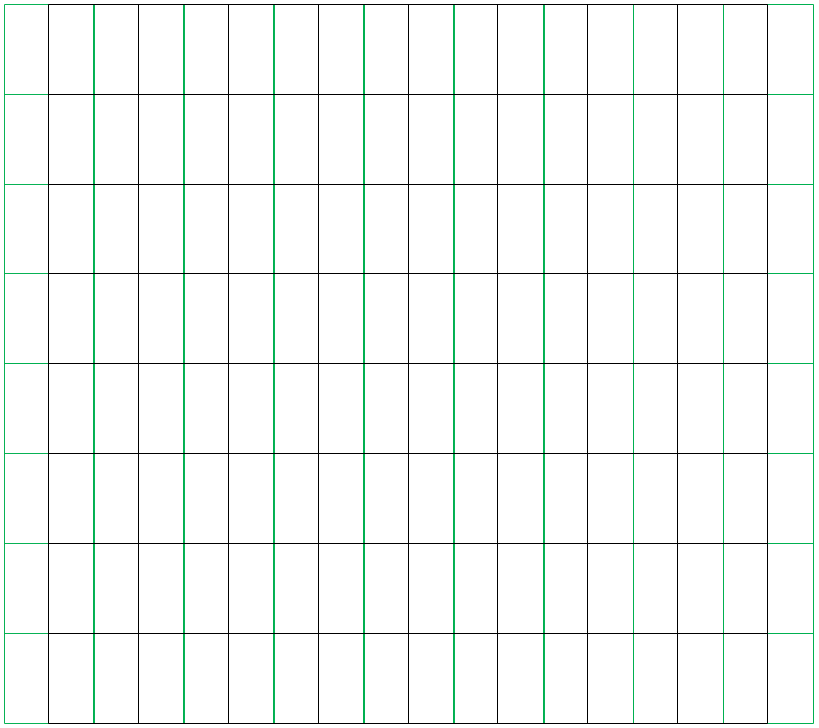
\includegraphics[width=200bp]{figure/grid.png}
	\caption{网格差别}
	\label{fig:diff-grid}
\end{figure}

\section{PBF流体仿真算法}


本文采用基于PBF(Position-basis fluid)的流体仿真算法。
在流体仿真领域,强制不可压缩性是一个很重要的特性,同时也是十分耗时的计算过程。
虽然最近的工作已经提高很效率,但对于实时应用来说还是不切实际的。
PBS是Miles和Matthias\upcite{Macklin2013Position}在2013年提出了一种融入
PBD(Position Based Dynamics)方法的迭代求解密度的方法,
通过求解一组位置约束,从而强制保证密度不变。
此方法可以实现类似SPH(Smoothed Particle Hydrodynamic)的仿真过程,
同时保留了几何关系的稳定性,最重要的是保持满足实时应用中对长时间步长的要求。
通过引入一个人工压力用来改善粒子的分布,创建表面张力并且降低传统SPH对邻居的需求。
最后通过应用涡旋约束作为速度处理来解决能量损失的问题。

其算法伪代码如算法 \ref{alg:pbf-algorithm} 所示。

\begin{algorithm}
  \caption{PBF算法}
  \label{alg:pbf-algorithm}
\begin{algorithmic}
\FORALL{粒子 $P_i$}
\STATE 应用外力更新加速度 $v_i \Leftarrow v_i + \Delta{}tf_{ext}(x_i) $
\STATE 计算预计位置$x_i^{*} \Leftarrow x_i + \Delta{} tv_i$
\ENDFOR
\FORALL{粒子 $P_i$}
\STATE 查找邻居粒子$N_i(x_i^*)$
\ENDFOR
\WHILE{迭代器 < 迭代次数}
\FORALL{粒子 $P_i$}
\STATE 计算$\lambda_i$
\ENDFOR
\FORALL{粒子 $P_i$}
\STATE 计算位置校正$\Delta{}p_i$
\STATE 执行碰撞检测和响应
\ENDFOR
\FORALL{粒子 $P_i$}
\STATE 校正位置$x_i^* \Leftarrow x_i^* + \Delta{}p_i$
\ENDFOR
\ENDWHILE
\FORALL{粒子 $P_i$}
\STATE 校正速度$v_i \Leftarrow \frac{1}{\Delta{}t}(x_i^*-x_i)$
\STATE 应用涡旋约束和XSPH粘性
\STATE 校正位置信息$x_i \Leftarrow x_i^*$
\ENDFOR
\end{algorithmic}
\end{algorithm}
\begin{figure}
	\centering
	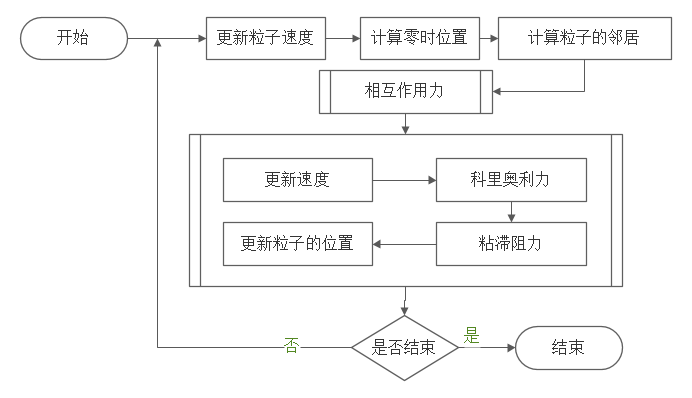
\includegraphics[width = 350bp]{figure/PBF-flow-chart.png}
	\caption{PBF流程图}
	\label{fig:pbf-flow-chart}
\end{figure}
在仿真循环过程中,首先是通过分析外力变化,分别校正粒子的速度和预计的位置;
其次是计算粒子在预期位置的邻居,通过执行碰撞检测和响应并校正预期位置,通过迭代计算直至收敛;
然后再根据预期位置和仿真前的位置校正速度,引用涡旋约束和人工粘性,最后校正粒子的位置。
流程图如下图\ref{fig:pbf-flow-chart}所示:


本流体仿真算法是本位论的重点研究内容,详细见第\ref{sec:fulid-simulation}部分。

\section{时序数据校准}

时序数据的校准时本论文的难点所在。此处只简单说明一些实现过程,
在技术难点和重点章节详细介绍本部分内容。

\section{基于LOD的多散射云绘制系统}

通过之前的工作,已经将WRF数据转化为粒子结构的云数据,
绘制时只要对粒子数据进行相应的调度之后就可以进行绘制,此阶段主要求解光线和粒子的相互作用,
同时确定粒子和粒子之间的相互作用,确定粒子入射光照强度以及粒子出射光照强度。
然而云作为一种参与介质,其内部的物理光照过程比较复杂,为了能够描述这种光线穿透云的光学现象,
本节主要介绍了三维云的光照模型基本原理以及优化求解适用于表面粒子的光照模型。

\subsection{相位方程}

下面解释相位方程的概念。当光线射入云粒子发生向外散射时,它可能被散射到任意的方向,
这取决于该粒子实际的光学性质,比如大小、形状、折射率等。光线向各个方向的分布通常是不均匀的。
相位方程则是对这个分布的定量描述,在给定入射方向$\omega$的前提下,
相位方程给出了散射到$\omega'$方向的能量占总能量的比例。如图\ref{fig:phase_function}所示,
$\varphi$表示$\omega$和$\omega'$的夹角,作为方程的自变量。
\begin{figure}
	\centering
	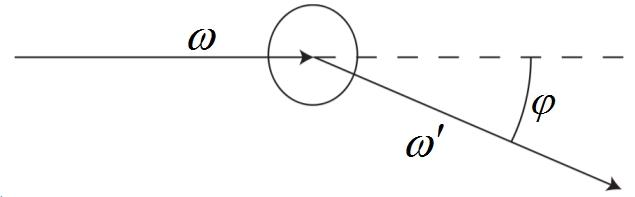
\includegraphics{figure/phase_function.jpg}
	\caption{相位函数示意图}
	\label{fig:phase_function}
\end{figure}

RayLeigh\upcite{StruttOn}和Mie\upcite{Mie1908Beitr}是两个经典的相位方程,
RayLeigh比较适合描述较小的粒子,不同波长的光交互过程相互独立,
很好的解释了天空呈现蓝色、晚霞以及彩虹的成因,
RayLeigh相位方程的形式如公式 \ref{equ:phase_function_ray} 所示,
其中$\lambda$表示光的波长,$\phi$表示入射光线和出射光线的夹角。
\begin{equation}
	\label{equ:phase_function_ray}
	p(\phi) = \frac{3}{4}\frac{(1+\cos^{2}\phi)}{\lambda^{4}}
\end{equation}

当粒子的尺寸大于光的波长时,Mie给出了更好的描述。它比RayLeigh方程的形式更加复杂,
计算复杂度很高,因此,也产生了很多近似的形式。
Henyey和Greenstein提出的模型\upcite{Henyey1941}是目前最常用的一种近似方法,
引入了各向异性因子$g$,它的形式如下:
\begin{equation}
	\label{equ:phase_function_henyey}
	p(\phi) = \frac{1}{4\pi}\frac{1-g^2}{(1-2g\cos\phi +g^2)^{\frac{3}{2}}}
\end{equation}

云由多种水汽粒子构成,主要有水、冰、雨、雪、霰等,
这些粒子占云的比重随云的海拔位置及天气环境发生改变。不同粒子与光的交互过程各不相同,
Wendling\upcite{Madronich1999The}通过模拟冰和水散射发生时的情况,
获取了它们之间的差异,如图\ref{fig:ice_water_phase_function}所示。
冰粒子尺寸较小,发生散射时侧面分布的能量相对较多,散射过程更加接近RayLeigh的描述。
而水粒子的尺寸则相对较大,绝大多数能量趋向于保持向前传播的趋势,更加符合Mie方程的描述。
\begin{figure}
\centering
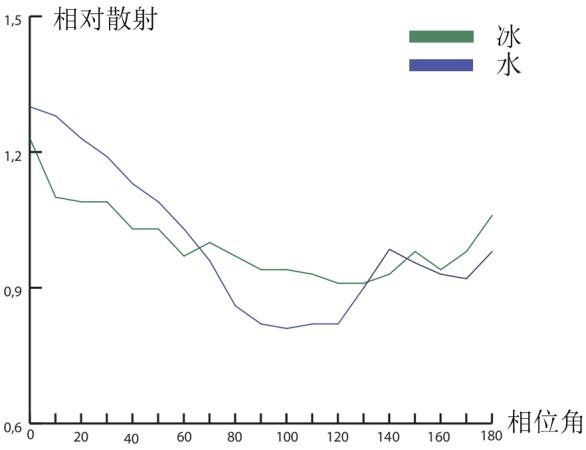
\includegraphics{figure/ice_water_phase_function.jpg}
\caption{冰水粒子相位函数对比}
\label{fig:ice_water_phase_function}
\end{figure}

由此可知,对云进行可视化时应当针对不同的粒子进行分别处理。
根据气象学对云的分类,近地面的云由于温度较高,多为水云,而冰云则多位于海拔较高的地方。
由于本文主要处理拍摄的自然图像,海拔较低,因此统一采用MIE方程进行近似。

\subsection{基本光照模型原理}

现实世界中,光线穿过类似于云这种不均匀参与介质时,会发生多种光学现象,如:
反射、折射、透射和散射等。同时光线来源也比较复杂,不仅包括太阳光,
还有可能包括天空背景光或地面反射光等。
而在所有这些光线之中,往往太阳光是光照强度比较大的一个光线来源,
但在某些特殊时间如太阳刚下山的黄昏时段,则是天空背景光的光照强度最强的时候。
针对不同的光线来源,其计算光照强度的方法也往往不同。

图\ref{fig:base_light_model}展示了不同光线对云粒子的入射光作用以及云粒子出射光对人眼的作用,
构成了基本的云光照模型。针对任意一个云中的粒子$X(t)$,其光照强度来源主要包括四种情况:
太阳光直接照射、其他粒子散射、天空背景光直接照射、地面反射光直接照射。
针对太阳光直接照射的光照强度,当太阳光光线以一定的入射角度进入云层后,
每穿透一个粒子,都会产生一定衰减,直至到达当前粒子。
针对其他粒子散射的光照强度,是由于光线在穿透不均匀参与介质时,由于光学传播较复杂,
发生了光线方向偏离的现象,经过多次的不规则作用,到达了当前粒子。
针对天空背景光以及地面反射光的光照强度,其计算过程与太阳光直接照射相似,
只是入射角度和入射强度有差别。

\begin{figure}
	\centering
	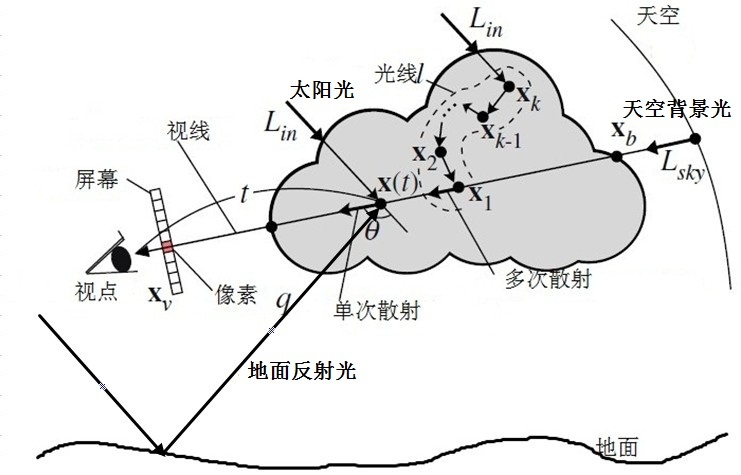
\includegraphics{figure/base_light_model.jpg}
	\caption{基本光照模型示意图}
	\label{fig:base_light_model}
\end{figure}

通过上述过程,云中的所有粒子所具有的光照强度可以计算得到,
而人眼看到的云的形态则可以描述为云中所有的粒子都可以发射光线至人眼。
因此沿着人眼的视线方向,将所有该条视线上的粒子光照强度进行叠加,
同时考虑叠加过程中的衰减,就可以得到三维云的最终绘制效果。

具体实现云的三维仿真通常包括两个步骤,light和render。
light是指确定云体中每点的能量,即计算光源(太阳光)以及周边邻居粒子经过散射照射到云粒子上,
使得云粒子具有的光照强度,render过程是指确定云最终屏幕成像的过程,
即将每一个云粒子看作是一个光源,投影到屏幕上产生的光强作用。

light的过程包括两种,单次散射和多次散射。
单次散射是指忽略入射方向之外的能量供给,即计算每点的能量时,
仅计算入射光沿原传播方向经过层层衰减后到达的能量。
多次散射则考虑附近其他粒子散射的综合作用。如图\ref{fig:base_light_model}所示,
多次散射计算$x_t$的能量需要考虑来自路径$x_1,x_2,x_3,x_4\dots{}\dots{}x_n$上贡献的能量。
在多次散射的定义中,仅考虑周围一个邻域中粒子的贡献,称为二次散射。
考虑周围粒子时同时考虑它接受的散射能量称为三次散射,依次类推。
多次散射是在单次散射的基础上使云体内的能量趋向于均匀的过程,
事实上,多次散射更加符合实际情况。但是实现的复杂度很高,一般都是采用一些近似的算法。

通过对相位方程的研究,Riley\upcite{Riley2004A}给出了一个相对科学又易于实现的近似方法,
由于前向散射($10^0$以内)的能量占水汽粒子散射总能量的$90\%$以上,
即粒子受到的散射影响主要来源于光源入射方向以及这个方向一个较小的夹角中。
因此,可以通过计算入射方向的一个圆锥邻域来代替多次散射。
而对于忽略掉的能量,则利用一个环境光常数进行补偿。

如图 \ref{fig:multiple_scattering_simplified_model} 所示。
为了进一步拟合实际光照过程,可以将这个提供主要能量的圆锥分为两个部分,
主要邻域和次要邻域。取$\theta{}=10^0$,则主要邻域的立体角为能量圆锥的一半$\theta{}/2$ ,
次要邻域的立体角为$\theta{}/4$ 。在主要邻域和次要邻域上分别选取平均分布的四个点,
作为能量的采样点。

\begin{figure}
\centering
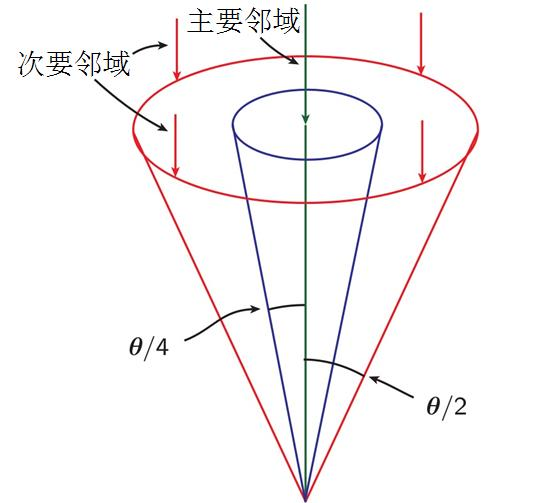
\includegraphics{figure/multiple_scattering_simplified_model.jpg}
\caption{多次散射简化模型}
\label{fig:multiple_scattering_simplified_model}
\end{figure}

\begin{equation}
\label{equ:multiple_scattering_simplified_function}
L_m(x)=L(x) + \sum{}L(\theta{}/2)p(\theta{}/2) + \sum{}L(\theta{}/4)p(\theta{}/4)
\end{equation}

如公式\ref{equ:multiple_scattering_simplified_function}所示,
多次散射的能量$L_m(x)$等于单次散射的能量$L(x)$与邻域贡献的叠加。
其中等号右边第二项表示主要邻域的贡献,第三项表示次要邻域的贡献,$p$表示相位方程。
而单次散射的能量$L(x)$则如下表示:
\begin{equation}
\label{equ:illumination}
L(x)=L_in(x)T(x_in,x)
\end{equation}

其中,$T(x_in,x)$表示$x$点沿入射光方向到云体边界的衰减,$x_in$则表示云体边界上的点。
$L(x)$也可由$x$和$x_in$的连线上距离$x$最近的一点进行计算。可以理解为能量沿入射方向进行层层衰减。
每一点的能量$L(x_{n+1})$都等于上一点$x_n$经过衰减后的能量。
如公式\ref{equ:extinction_transfer_function}所示。
\begin{equation}
\label{equ:extinction_transfer_function}
L(x_{n+1})=L(x_n)T(x_n,x_{n+1})
\end{equation}

需要说明的是,虽然近似的认为相位方程对不同波长的光具有同样的表现,但是衰减系数确是相互独立的。
即可以认为衰减系数$\sigma$是一个衰减系数集合。以RGB通道为例,
$\sigma$等于$\{\sigma_r,\sigma_g,\sigma_b\}$。本文接下来都是在RGB颜色空间进行相关的计算。
因此,无论是light还是render的过程,都需要在这三个通道中分别计算。

确定了云体能量之后,就可以进行render的过程计算最终的屏幕成像。为了对多次散射进行补偿,
在绘制过程引入环境光常数$L_amb(\lambda)$,作为能量的附加值进行计算。
具体过程如公式
所示:
\begin{equation}
\label{equ:multiple_scattering_compensation}
I_\lambda(q) = (L_{sky}(\lambda)T_\lambda(x_b,x_f)+
\int_{x_b}^{x_f}\beta\sigma_\lambda(x)p(\Omega)T_\lambda(x,x_f)(L_\lambda(x)+L{amb}(\lambda))
T_\lambda(x_v,x_f)
\end{equation}

其中,$q$表示屏幕像素,$L_{sky}(\lambda)$表示天空提供的背景能量,$\lambda{}={R,G,B}$。
如图\ref{fig:render_principle}所示,依据透视投影原理,
$x_f$表示视线穿过云体与云相交的第一个点,$x_b$表示相交的最后一个点,
 $x_v$表示视线发出点,$T_\lambda(x_v,x_f)$表示能量进入眼睛之前在空气中发生的衰减,
$T_\lambda(x,x_f)$表示能量从$x$到$x_f$点处发生的衰减,$L_\lambda(x)$表示$x$点处的能量,
$I_\lambda$表示图像平面,$\Omega$表示入射光与视线的夹角。

\begin{figure}
\centering
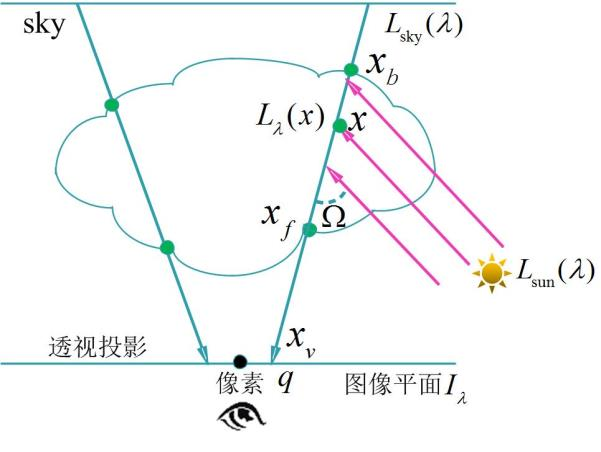
\includegraphics{figure/render_principle.jpg}
\caption{绘制过程原理图}
\label{fig:render_principle}
\end{figure}








